\documentclass[11pt,a4paper]{article}
\usepackage[a4paper,top=40mm,right=30mm,left=30mm,bottom=20mm]{geometry}
\usepackage[utf8]{inputenc}
\usepackage{amsmath}
\usepackage{amsfonts}
\usepackage{amssymb}
\usepackage{graphicx}
\author{Prakash Gautam}
\begin{document}
\begin{titlepage}
	\begin{center}
		\begin{Huge}
			Tribhuvan University\\
			
\includegraphics[scale=1.6]{./Images/logo.png}\\
			Institute of Engineering\\
			Pulchowk Campus\\[1.6cm]		
		\end{Huge}
		\textbf{A\\
		Mid Term Report On\\
		Tracking and Acciedent Alert System}\\[1cm]
		\textbf{Submitted To:}\\
		Department of\\
		Electronics and Computer\\Engineering\\[1.6cm]
	
		\textbf{Submitted By:}\\
		Arjun Upadhyay (068BEX407)\\
		Bibek Shah (068BEX410)\\		
		Bijay Neupane (068BEX412)\\
		Bishal Dangal(068BEX415)\\[1.5cm]
		\today	
	\end{center}
\end{titlepage}
\pagenumbering{roman}
\tableofcontents
\newpage
\abstract{ This project has been done as a part of syllabus of minor project (VI semester). We have designed a tracking and accident alert system to fulfill the requirement of the system. The project is aimed to design and development of the embedded system that is used to control/prevent the theft of the vehicle. The main objective of the design  is to protect from unauthorized access , through entering the protected password and intimate the status of same vehicle to authorize person using Wireless Networking , which can be further enhanced with remote  networking . Also it is intended to detect the accident and notify to the concerned authority 


The proposed work is attempt to design a tracking unit to determine the precise location of a object  (vehicles) and using  networking technology this information can be transmitted to the user. The project comprises of embedded system that is equipped with GPS and networking model (represented by WLAN or other form of wireless networking ) , with enhacement forms remote networking (such as GSM ) along with beaglebone ARM microcontroller installed in vehicle. If the password is sent by the owner , it automatically stops the vehicle and we can do for the different works, or it can provide the real time control. Thus when the accident is detected the tracked location can be sent to central emergency dispatch server. 
}


\newpage

\pagenumbering{arabic}

\section{Introduction}
In these days, automobile thefts are increasing at an alarming rate all over the world.  The commercially available anti-theft vehicular systems are very expensive. Here, we make an attempt to develop an instrument based on BEAGLEBONE ARM microcontroller and operated using LAN networking . \\ 

 During vehicle motion, its real-time parameters such as location are reported by Networking. The system takes advantage of wireless technology in providing powerful management transportation engine. The use of Networking and GPS technologies allows the system to track vehicle and provides the most up-to-date information about ongoing trips. This system finds its application in real time traffic surveillance. \\
 
 It could be used as a valuable tool for real time traveler information, congestion monitoring, and system evaluation. An intelligent, automated vehicle tracking system can resolve following problems such as, late arrivals to scheduled, improper use of company time and resources, unsafe driving habits, assigned routes, inefficient dispatching. This can lead to better traffic flow modeling and a better understanding of driver behavior. \\
 
 This project includes various features like ingenuity, simplicity of design and easy implementation. It is completely  integrated so that once it is implemented in all vehicles (after enhancement ) then it is easy to track vehicle any time. 


\section{Objectives}
The primary objectives of the project are as follows.
\begin{enumerate} 
   \item To carry out small scale project to develop hands of experience of working  in
  \item To implement the theoritical knowledge in practical field , and hence develop      
        the general experience of real world project.
   \item Co-operation , teamwork and work synchronization among the project 
       members , which indeed proves beneficial in days to come.
   \item To develop the knowledge of application development platforms and 
        tools(c/c++,proteus and various other platforms)
   \item To meet the syllabus prescribed by IOE , TU.
\end{enumerate}
Along with these objectives main objectives of this project are:
\begin{enumerate}

   \item To design the Tracking and Accident Alert System to facilate the anti-theft Operation and minimize the fatalities due to accident.
  \item Addition of proper user interface like push button, LED indicators etc.

\end{enumerate}
\newpage

\section{Block Diagram}
The Block diagram of our system is depicted in the following Figure \ref{fig:BlockDiagram}.
\begin{figure}[h]	
	\centering
	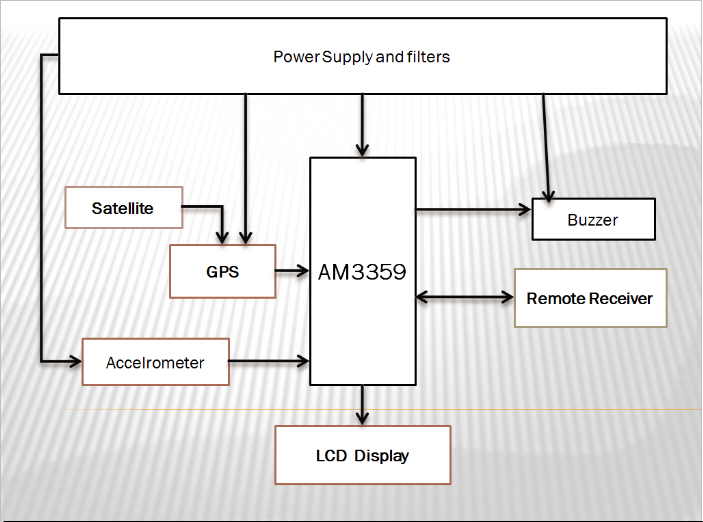
\includegraphics[scale=.35]{BaleImages/BlockDiagram.png}
	\caption{Beagle Bone}
	\label{fig:BlockDiagram}
\end{figure}


\section{Hardware Selection}
Different hardware components used in the project are described in brief in the following section. \textit{Beagle Bone Black} is the primary hardware used and the major hardware are LCD, mma7631L accelerometer.
\subsection{Beagle Bone}
Beagle bone is a a low cost community-supported development paltform for developers and hobbystis. It has AM335x 1GhHs Corted-A8 Arm Processor.
\begin{figure}[h]	
	\centering
	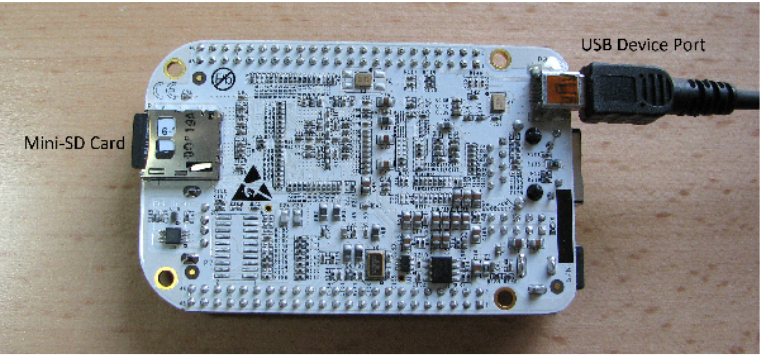
\includegraphics[scale=.35]{BaleImages/beagleBone.png}
	\caption{Beagle Bone}
	\label{fig:BeagleBone}
\end{figure}

\subsection{Acclerometer}
We have uses MMA731L acclerometer to sense the accleration, it gives analog signal according to the accleration it senses ranging from 0.5 to 1.8 volts. The analog signal is then converted to digital signal to be processed by the beagle bone.

\begin{figure}[hbtp]
\centering
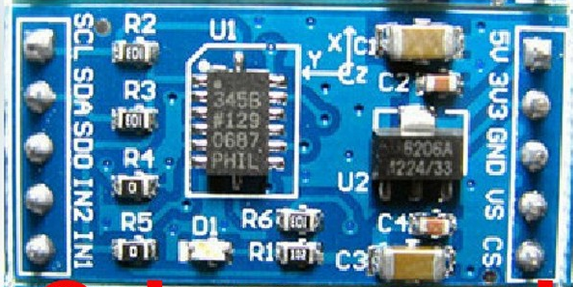
\includegraphics[scale=.4]{BaleImages/Acclerometer.png}
\caption{USBasp Programmer}
\end{figure}

\subsection{Skylab GPS-6M001415}
It sends data through NMEA Protocal and the data will be proceessed in the Beagle Bone. It is used to find the position and the velocity of the vechicle under survillence.


\section{Work Completed}
Due to the unviability of the devices like GPS and accelerometer we didn’t have a fast head start. Since the beagle bone is very sensitive to the amount of current a direct connection for the alarm was not appropriate. So, we had to use the transistor and pull up resistor to limit the amount of current and also fit our purpose of providing an output. Thus, the problem of providing output is eradicated.
Similarly, a power supply of 5V and maximum 400mA is almost completed. Similarly the required filters are also made.
The work of accelerometer sensor is completed only spikes of output from sensors are yet to be handled though.  
				

\section{Work Remaining}
The programming part of GPS is yet to be done. The feedback form of power supply with amplifier and filter is in progress. Similarly, PCB layout of the whole circuit is to be done. Data transmission portion is also remaining. And, if we get the time then LCD display of the complete output is also a priority.

\section{Conclusion}
We are very much confident that we can complete the project in time. This project, though not completed yet, has taught us a lot of things on micro-controller programming. Though only the beginning of , this project has made us pretty excited on building some hardware architecture. Beginning with almost zero knowledge on embeded system based hardware, this project has made us go through so many e-books and video tutorials. Therefore, we have helped ourselves with self learning and some sort of combined study with the project members.


Though we do not have any hard and fast schedule for accomplishing the project, for the time being we are ahead of what could have been an ideal schedule for this project. The solutions of the problems are being dealt with pretty effectively and we are more than confident that this project will be completed in time.
Apart from the things we learn through this project, we believe this project can also become a quite applicable one in modern day technology. 

\begin{thebibliography}{99}
\bibitem{} \textit{http://beaglebone.org/}

\bibitem{} Wikipedia the open internet library \emph{http://en.wikipedia.org/wiki/beaglebone}
\bibitem{} \emph{Derekmolley.com}
\bibitem{} Texas Instruments \emph{http://ti.com/}
\end{thebibliography}
\end{document}